\subsection*{A Analog simulation graphs}
\addcontentsline{toc}{subsection}{A Analog simulation graphs}
\label{sec:analogSimulationGraphs}

\begin{figure}[H]
    \centering
    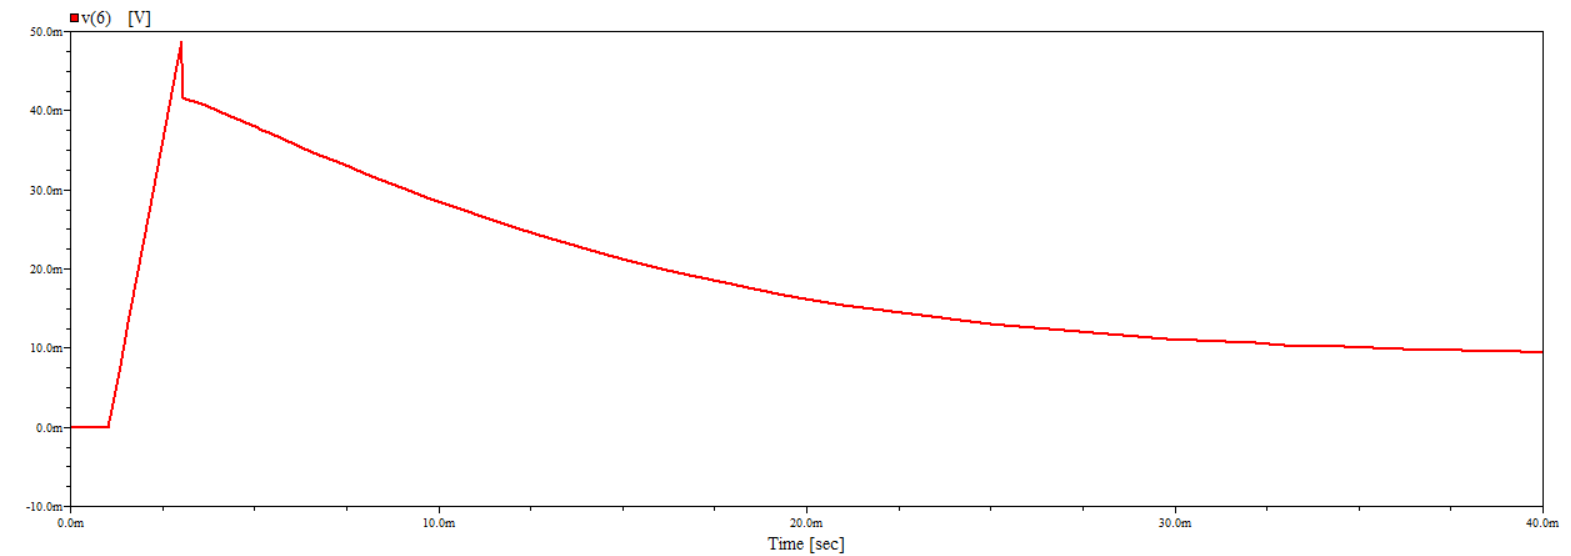
\includegraphics[width=\textwidth]{graphs/minExp_minLight.png}
    \caption{Minimum exposure time - minimum light}
    \label{fig:min-min}
\end{figure}

\begin{figure}[H]
    \centering
    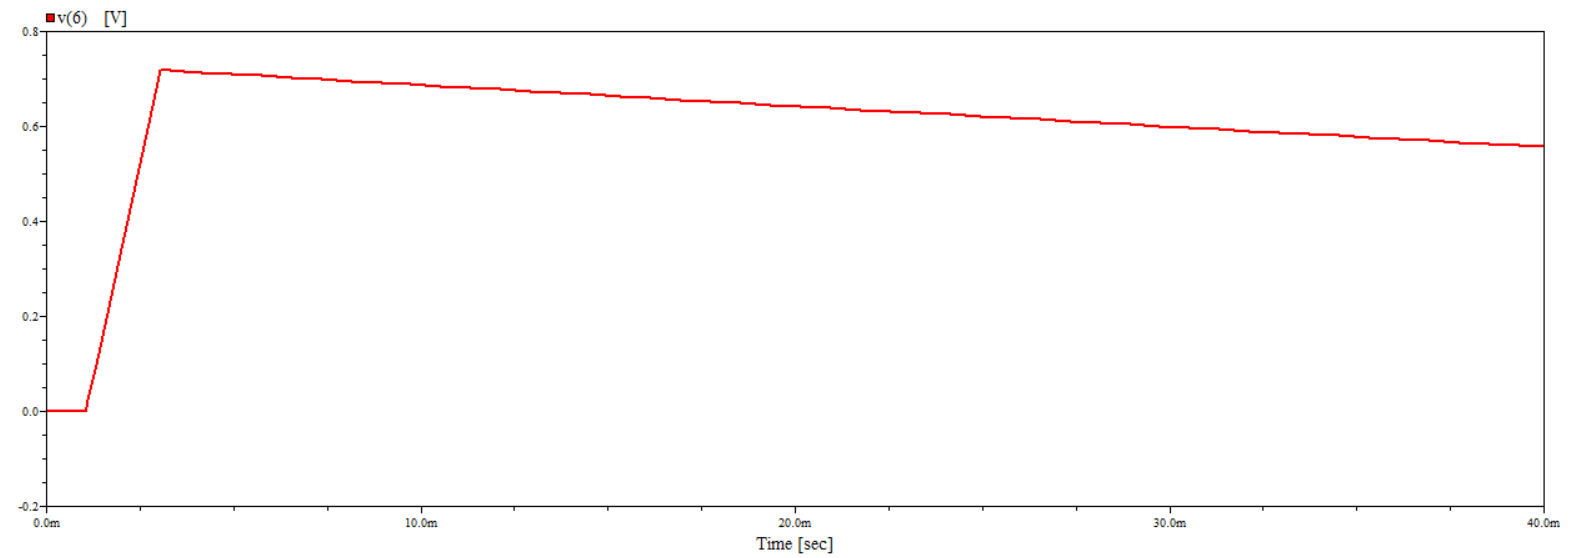
\includegraphics[width=\textwidth]{graphs/minExp_maxLight.png}
    \caption{Minimum exposure time - maximum light}
    \label{fig:min-max}
\end{figure}

\begin{figure}[H]
    \centering
    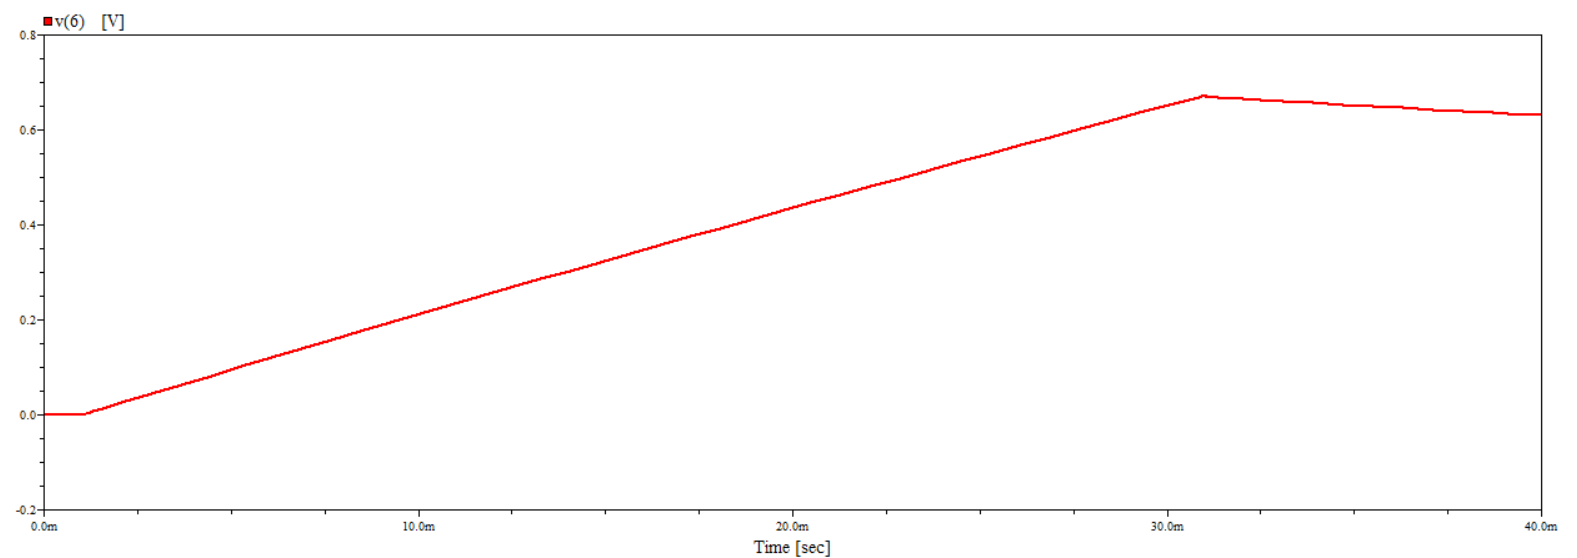
\includegraphics[width=\textwidth]{graphs/maxExp_minLight.png}
    \caption{Maximum exposure time - minimum light}
    \label{fig:max-min}
\end{figure}

\begin{figure}[H]
    \centering
    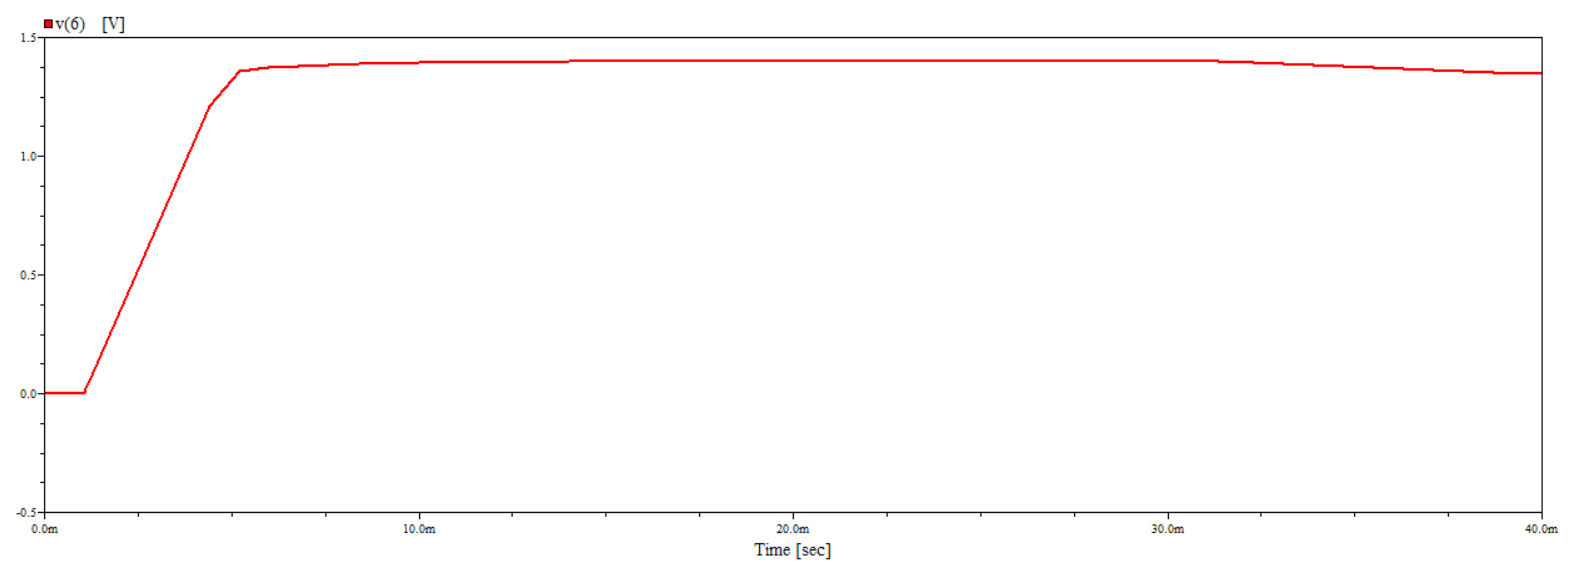
\includegraphics[width=\textwidth]{graphs/maxExp_maxLight.png}
    \caption{Maximum exposure time - maximum light}
    \label{fig:max-max}
\end{figure}

\begin{figure}[H]
    \centering
    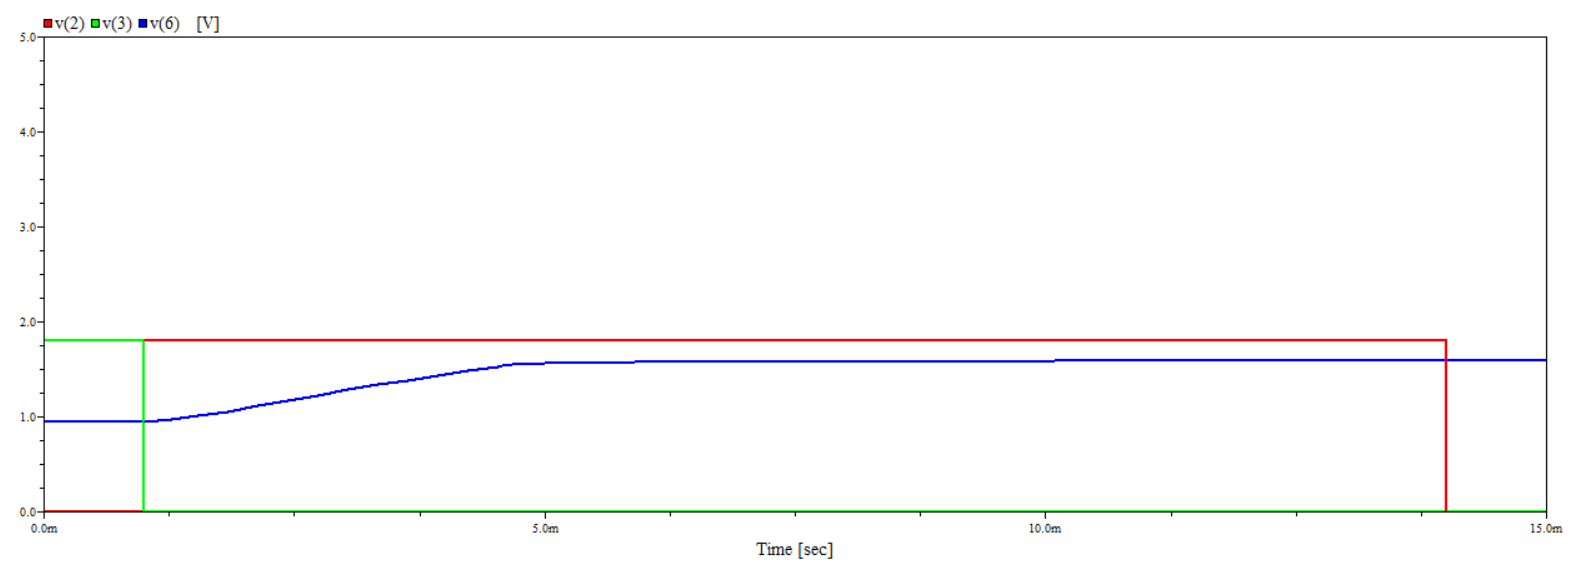
\includegraphics[width=\textwidth]{graphs/m3AndActiveLoadSim.png}
    \caption{Simulation for maximizing dynamic range of M3 and active load.}
    \label{fig:m3AndActiveLoadSim}
\end{figure}

\begin{figure}[H]
    \centering
    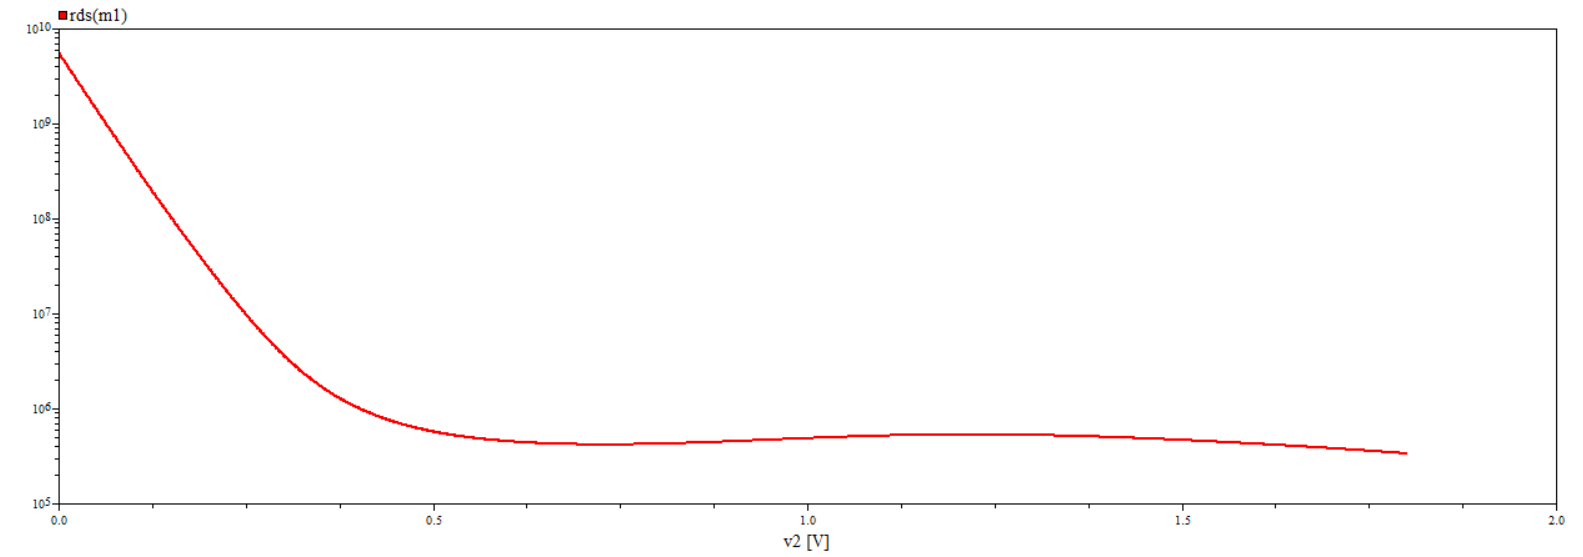
\includegraphics[width=\textwidth]{graphs/corner_ff_simulation.png}
    \caption{FF corner simulation of $R_{DS}$ of NMOS switch as function of $V_{GS}$. $V_{DS} = 1.8\mathrm{V}$.}
    \label{fig:ff}
\end{figure}

\begin{figure}[H]
    \centering
    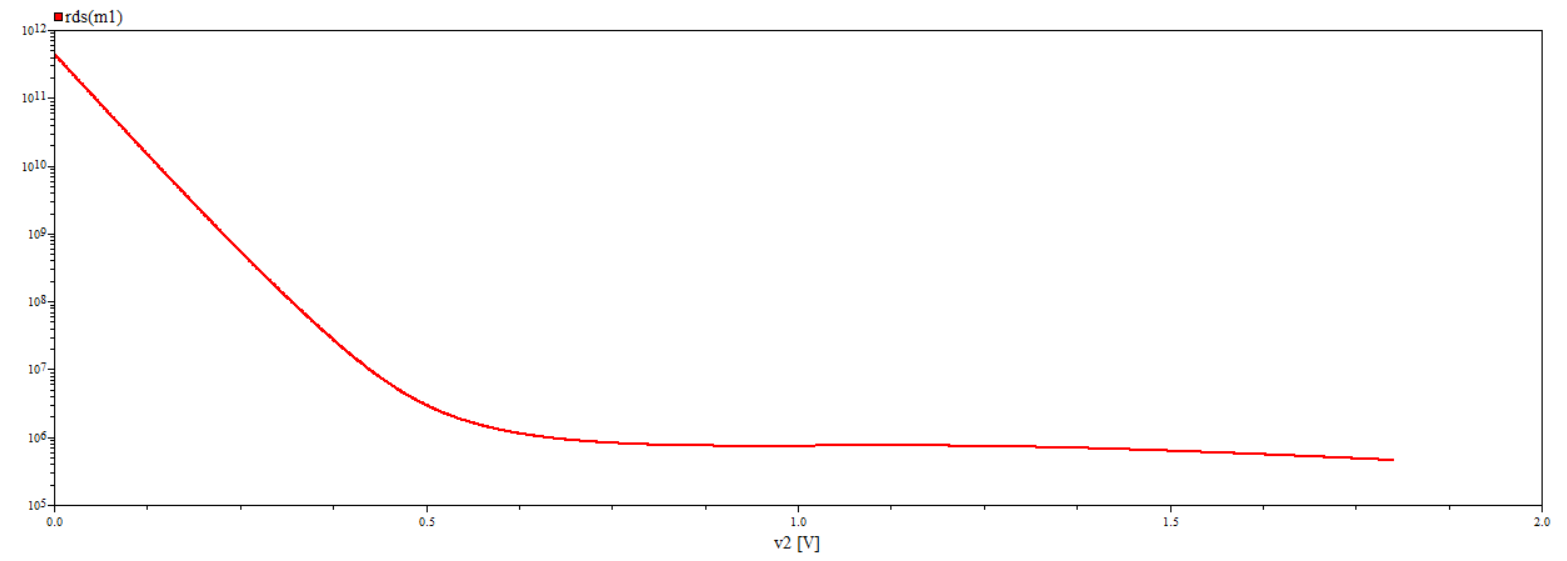
\includegraphics[width=\textwidth]{graphs/corner_tt_simulation.png}
    \caption{TT corner simulation of $R_{DS}$ of NMOS switch as function of $V_{GS}$. $V_{DS} = 1.8\mathrm{V}$.}
    \label{fig:tt}
\end{figure}

\begin{figure}[H]
    \centering
    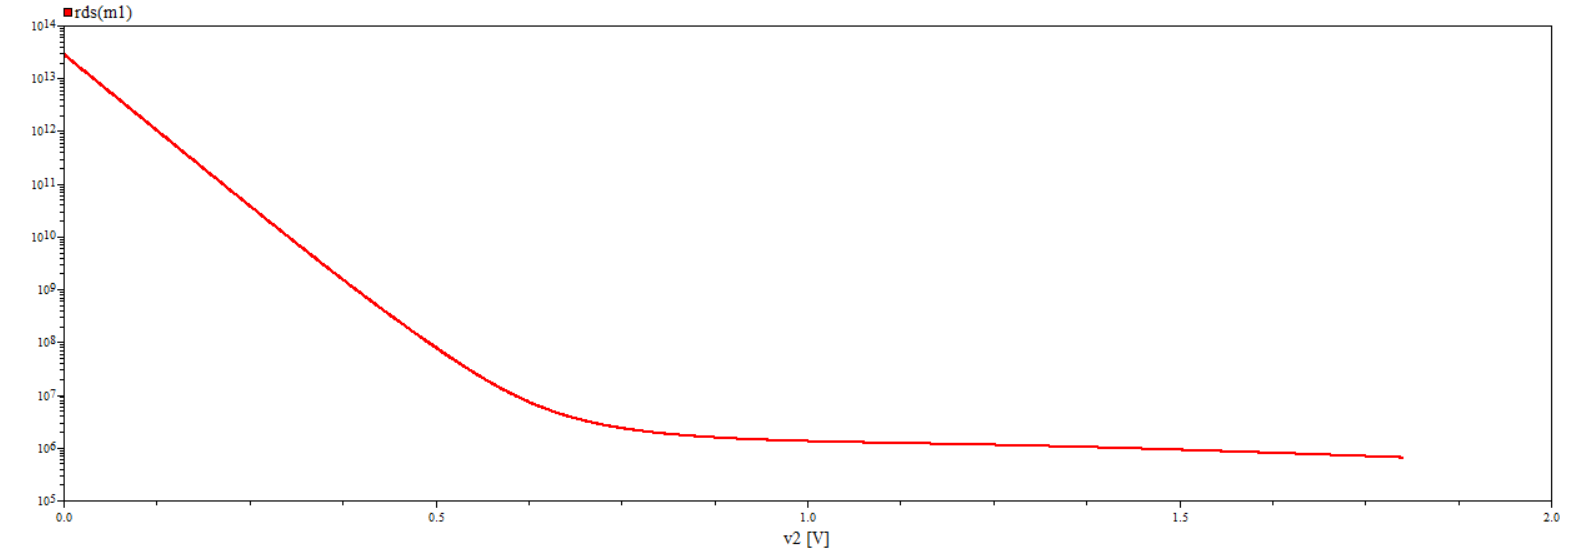
\includegraphics[width=\textwidth]{graphs/corner_ss_simulation.png}
    \caption{SS corner simulation of $R_{DS}$ of NMOS switch as function of $V_{GS}$. $V_{DS} = 1.8\mathrm{V}$.}
    \label{fig:ss}
\end{figure}

\begin{figure}[H]
    \centering
    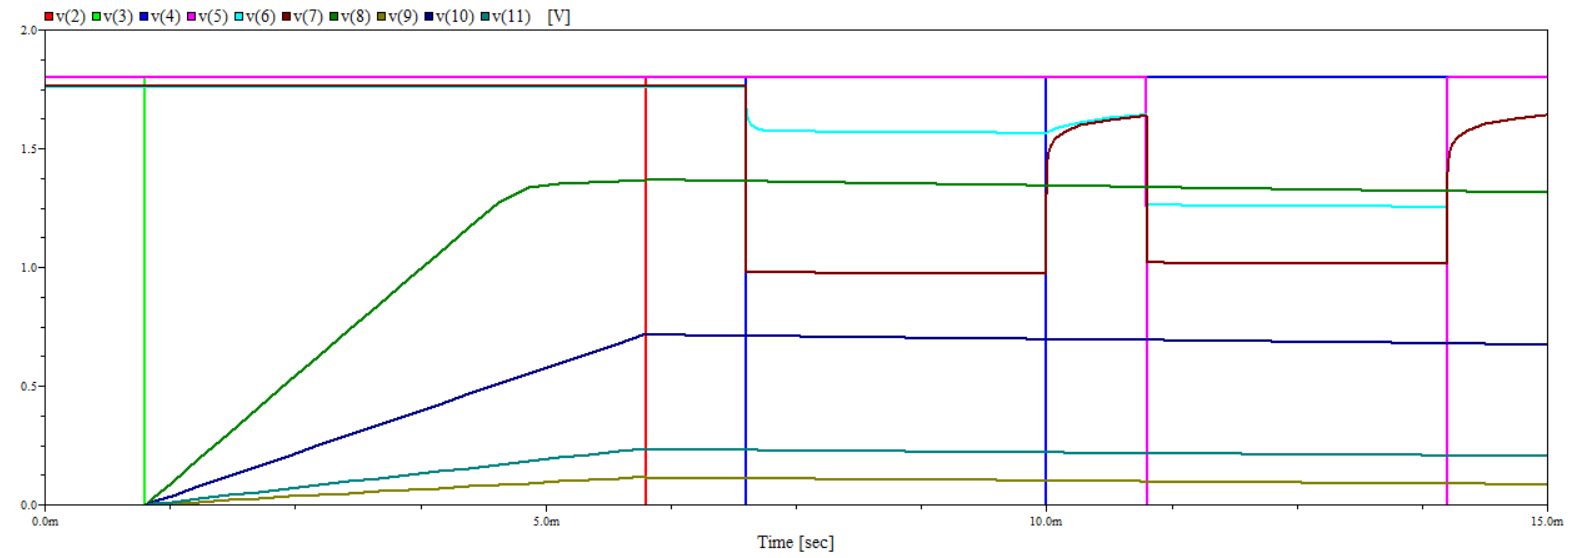
\includegraphics[width=\textwidth]{graphs/analogWaveform.png}
    \caption{Simulation of analog circuit. The color(node nr)'s are: red(2): EXPOSE, light green(3): ERASE, blue(4): NRE\_1, magenta(5): NRE\_2, light blue(6): OUT1, brown(7): OUT2, dark green(8): $V_{C11}$, mustard(9): $V_{C12}$, dark blue(10): $V_{C21}$, teal(11): $V_{C22}$.}
    \label{fig:analogWaveform}
\end{figure}

\begin{figure}[H]
    \centering
    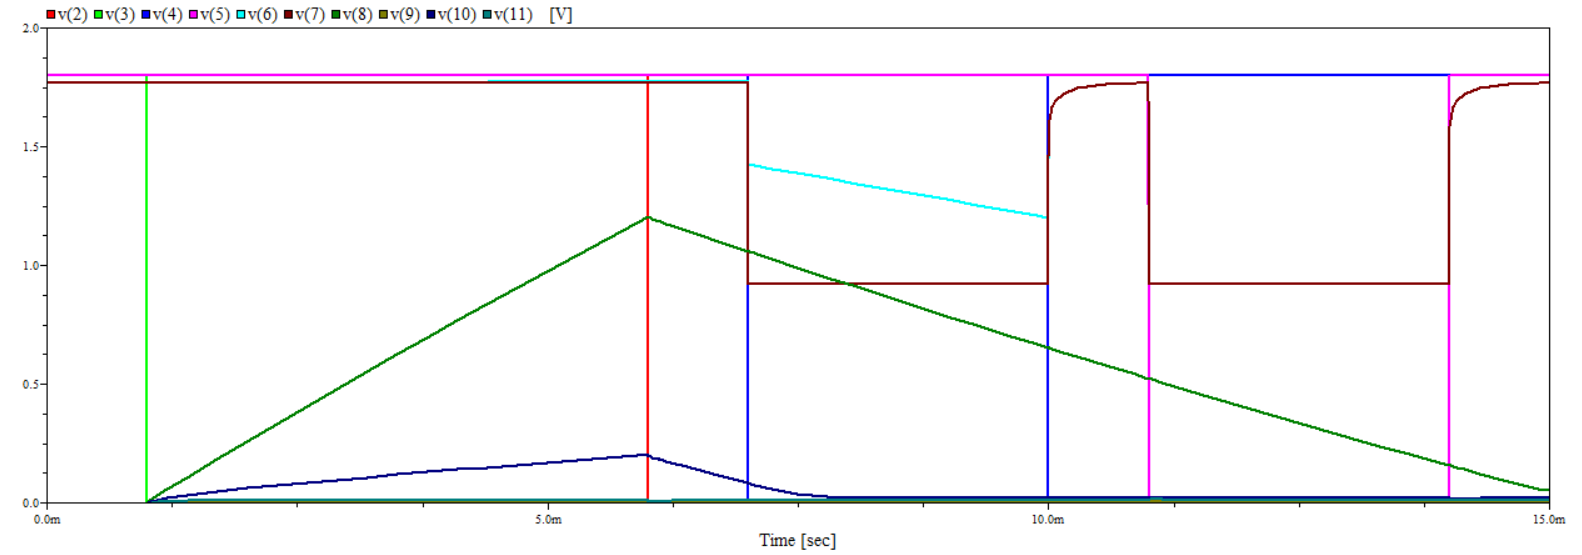
\includegraphics[width=\textwidth]{graphs/analogWaveform_ff.png}
    \caption{FF corner simulation of full analog circuit. Colors are the same as in figure \ref{fig:analogWaveform}.}
    \label{fig:ffFull}
\end{figure}

\begin{figure}[H]
    \centering
    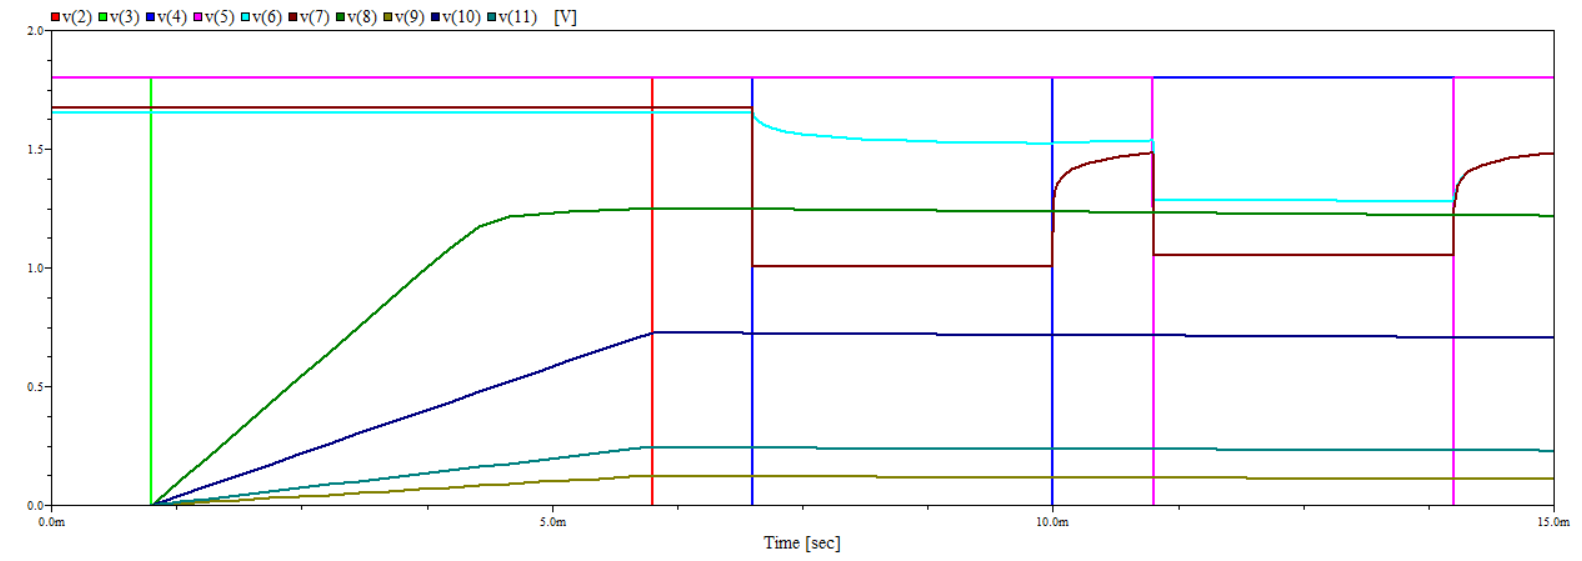
\includegraphics[width=\textwidth]{graphs/analogWaveform_ss.png}
    \caption{SS corner simulation of full analog circuit. Colors are the same as in figure \ref{fig:analogWaveform}.}
    \label{fig:ssFull}
\end{figure}
